% mnras_template.tex
%
% LaTeX template for creating an MNRAS paper
%
% v3.0 released 14 May 2015
% (version numbers match those of mnras.cls)
%
% Copyright (C) Royal Astronomical Society 2015
% Authors:
% Keith T. Smith (Royal Astronomical Society)

% Change log
%
% v3.0 May 2015
%    Renamed to match the new package name
%    Version number matches mnras.cls
%    A few minor tweaks to wording
% v1.0 September 2013
%    Beta testing only - never publicly released
%    First version: a simple (ish) template for creating an MNRAS paper

%%%%%%%%%%%%%%%%%%%%%%%%%%%%%%%%%%%%%%%%%%%%%%%%%%
% Basic setup. Most papers should leave these options alone.
\documentclass[a4paper,fleqn,usenatbib]{mnras}

% MNRAS is set in Times font. If you don't have this installed (most LaTeX
% installations will be fine) or prefer the old Computer Modern fonts, comment
% out the following line
% Depending on your LaTeX fonts installation, you might get better results with one of these:
%\usepackage{mathptmx}
%\usepackage{txfonts}

% Use vector fonts, so it zooms properly in on-screen viewing software
% Don't change these lines unless you know what you are doing
\usepackage[T1]{fontenc}
\usepackage{ae,aecompl}


%%%%% AUTHORS - PLACE YOUR OWN PACKAGES HERE %%%%%

% Only include extra packages if you really need them. Common packages are:
\usepackage{graphicx}	% Including figure files
\usepackage{amsmath}	% Advanced maths commands
\usepackage{amssymb}	% Extra maths symbols

%%%%%%%%%%%%%%%%%%%%%%%%%%%%%%%%%%%%%%%%%%%%%%%%%%

%%%%% AUTHORS - PLACE YOUR OWN COMMANDS HERE %%%%%

% Please keep new commands to a minimum, and use \newcommand not \def to avoid
% overwriting existing commands. Example:
%\newcommand{\pcm}{\,cm$^{-2}$}	% per cm-squared

%%%%%%%%%%%%%%%%%%%%%%%%%%%%%%%%%%%%%%%%%%%%%%%%%%

%%%%%%%%%%%%%%%%%%% TITLE PAGE %%%%%%%%%%%%%%%%%%%

% Title of the paper, and the short title which is used in the headers.
% Keep the title short and informative.
\title[Short title, max. 45 characters]{MNRAS \LaTeXe\ template -- title goes here}

% The list of authors, and the short list which is used in the headers.
% If you need two or more lines of authors, add an extra line using \newauthor
\author[K. T. Smith et al.]{
Keith T. Smith,$^{1}$\thanks{E-mail: mn@ras.org.uk (KTS)}
A. N. Other,$^{2}$
Third Author$^{2,3}$
and Fourth Author$^{3}$
\\
% List of institutions
$^{1}$Royal Astronomical Society, Burlington House, Piccadilly, London W1J 0BQ, UK\\
$^{2}$Department, Institution, Street Address, City Postal Code, Country\\
$^{3}$Another Department, Different Institution, Street Address, City Postal Code, Country
}

% These dates will be filled out by the publisher
\date{Accepted XXX. Received YYY; in original form ZZZ}

% Enter the current year, for the copyright statements etc.
\pubyear{2015}

% Don't change these lines
\begin{document}
\label{firstpage}
\pagerange{\pageref{firstpage}--\pageref{lastpage}}
\maketitle

% Abstract of the paper
\begin{abstract}
This is a simple template for authors to write new MNRAS papers.
The abstract should briefly describe the aims, methods, and main results of the paper.
It should be a single paragraph not more than 250 words (200 words for Letters).
No references should appear in the abstract.
\end{abstract}

% Select between one and six entries from the list of approved keywords.
% Don't make up new ones.
\begin{keywords}
keyword1 -- keyword2 -- keyword3
\end{keywords}

%%%%%%%%%%%%%%%%%%%%%%%%%%%%%%%%%%%%%%%%%%%%%%%%%%

%%%%%%%%%%%%%%%%% BODY OF PAPER %%%%%%%%%%%%%%%%%%

\section{Introduction}

This is a simple template for authors to write new MNRAS papers.
See \texttt{mnras\_sample.tex} for a more complex example, and \texttt{mnras\_guide.tex}
for a full user guide.

\cite{Tweb}.

\section{Illustris Simulation}
Illustris-1, also known simply as Illustris, is a highly resolved
cosmological simulation. It reproduces large-scale statistical
features of the Universe, such as the galaxy population of massive
clusters, as well as small-scale properties such as the morphology of
galaxies and detailed values for their stellar and gas content.\\ 

This was achieved by following the evolution of $2 \times 1820^3$ elements with dark mass resolution of $m_{\text{DM}} = 6.26\cdot 10^6\text{M}_{\odot}$ and initial baryonic mass resolution of $\overline{\text{m}_\text{b}}=1.26\cdot 10^6\text{M}_{\odot}$ from a glass-like configuration in a periodic box of $106.5\text{Mpc}$. The $\Lambda \text{CDM}$ cosmology of this run follows: $\Omega_\Lambda=0.7274$, $\Omega_\text{m}=0.2726$, $\Omega_\text{b}=0.0456$, $\sigma_\text{s}=0.0809$, $\text{n}_\text{s}=0.963$ \& $\text{H}_0=70.4\text{kms}
^{-1}\text{Mpc}^{-1}$ which is consistent with the (last) Anisotropy
Probe (WMAP)-9 \cite{AnisotropyProbe}. Illustris has a constant
spatial resolution of $1.4\text{kpc}$ for DM particles in comoving
units, and for baryonic particles it has the same spatial resolution
of DM for $\text{z}\geq 1$, which is later modified to $0.7\text{kpc}$
in physical units for the rest of the simulation. \\ 

The evolution in time was performed with the hydrodynamic code AREPO
\cite{arepo}, which combines a moving Voronoi tessellation with the
finite volume approach. Included in the evolution algorithm, there are
galaxy formation models which account for the evolution of stars and
SMBHs. Specifically, the physics followed by this model includes
energetic feedback from supermassive black holes and supernovae, as
well as stellar evolution and chemical enrichment. This level of
detail in Illustris is advantageous for the analysis of the effect of
the environment in barionic properties of galaxies. This level of resolution is hard to find
among other simulations, i.e. post-processed runs with semi-analytical
models which do not directly simulate baryons.(Expand) Describe Arepo more\\ 

The output of this simultaion consists of 136 snapshots. 61 of
them were taken at $z < 3$ spaced with a cosmological scale factor
$\Delta a \approx 0.02$. The remaining 75 were taken at $z > 3$
with spacing $\Delta a \approx 0.01$. Each snapshot was post-processed
with a modified version of FOF \cite{FOF} to identify DM haloes with
more than 32 particles using a linking length of 0.2 times the mean
particle separation. Each output group from the 7,713,601 post-processed halos (FOF) is analyzed with the SUBFIND
algorithm \cite{subfind} to generate, at z=0,
and 4,366,546 (sub)halo catalogues with their respective
characterization properties. \\ 

(HERE TALK ABOUT ILLUSTRIS-2,3 FOR RESOLUTION PURPOSES)

\section{The method}

The principal purpose of this work is to verify if the results
obtained observationally by Jones et al. \cite{jones1} are supported
by a similar analysis in the cosmological simulation Illustris. Specifically, we focus on the (small-scale) environment definition of the $3^{rd}$ nearest neighbor, which we want to adapt as closely as possible to our computational application.\\ 

\subsection{The $3^{rd}$ nearest neighbor definition of environment}

Jones et al. \cite{jones1} analyses the
dependence of the Schechter parameters on the cosmological
environment. To obtain a quantification of said cosmological
environment, they calculated for each galaxy in the studied survey the
projected distance in the sky to the third nearest neighbor,
filtrating candidate neighbors by their radial velocity relative to the
reference galaxy. According to Hubble's law, this effectively
restricts the candidate galaxies to a smaller radial range, reducing
apparent closer galaxies arising from the projection method. The
radial relative velocity cut was chosen to be $450km/s$. In addition to this,
a photometrics pre-selection was performed, selecting galaxies whose
r-filter magnitude was above $-19$ (VERIFY).\\  

Once quantified the environment with the distance to the 3rd nearest
neighbor definition they divided the group in four quartiles according this quantity. For each
quartile, the respective HIMF was calculated, and with this, a
Schechter fit was obtained. The analysis was specifically performed
over the Schechter parameters of the Knee-mass and the faint-end
slope. (Some observational adjustments for the Schechter functions were performed)  \\ 
 
As we want to replicate as closely as possible the method effectuated by Jones et. al
\cite{jones1}, we use the same specifications to calculare the environment.
 We perform the analysis of the Schechter functions to gas, DM, stellar and BH mass functions.
 However, we do not perform it directly on HIMFs because this would require some extense calculations.
  We take the gas mass function as a first approximation.
 As Illustris is a cosmological simulation, it is subject to resolution biases.
The most important bias in this study is related to the minimum mass of discrete elements in the simulation. 
Each mass considered here is subject directly or indirectly this resolution restriction, and the effect it causes is specially evident in the produced mass functions. 
We used Illustris-2,3, which are less resoluted copies of Illustris-1, to show this effect on the mass functions \fig{resolution effects}. 
Taking this into account, mass functions are heavily affected for masses below a certain cut and for this reason, only galaxies above said cut are considered in this study. This mass cut has no aparent systematical way to be calculated and therefore, we performed the cut having into account the performance of the respective Schechter fit.\\

\subsection{The cosmic web method}
To complement and verify the analysis performed with the third nearest neighbor
method, we chose a complementary method of completely different nature. 
The chosen method was developed by Forero et al. \cite{forero1}. 
It uses the Hessian \ref{eq:hessian} of
the gravitational potential obtained from the DM density field to classify
galaxies into four morphological environments.\\  

\begin{equation}
E =  mc^2
\label{eq:hessian}
\end{equation}

Specifically, we diagonalize the Hessian matrix obtaining three eigenvalues. 
These eigenvalues determine the concavity of the gravitational potential on the principal axes, at each point. We use these eigenvalues to interpret the tendence of mass to cluster with reference with some given threshold $\lambda$. 
Eigenvalues bigger than $\lambda$ are interpreted as a local tendence of mass to expand? in the respective eigenaxes, and viceversa. 
With this characterization, clusters, sheets, fillaments and voids can be defined with the number of axes above $\lambda$.
Forero et. al. found in \cite{forero1} that the critical value that better reproduces the correct morphological pulations was $\lambda = 0.2$. \\

With these specifications, we could obtain mass functions for galaxies belonging to clusters, fillaments and sheets. The amount of galaxies belonging to voids was strongly affected by the mentioned mass cuts and could not produce reasonable mass functions to analyze.


\section{Results}
\subsection{Preliminaries}

\subsection{Mass functions comparison}

Figures and tables should be placed at logical positions in the text. Don't
worry about the exact layout, which will be handled by the publishers.

Figures are referred to as e.g. Fig.~\ref{fig:example_figure}, and tables as
e.g. Table~\ref{tab:example_table}.

% Quartiles gas
\begin{figure}
	% To include a figure from a file named example.*
	% Allowable file formats are eps or ps if compiling using latex
	% or pdf, png, jpg if compiling using pdflatex
	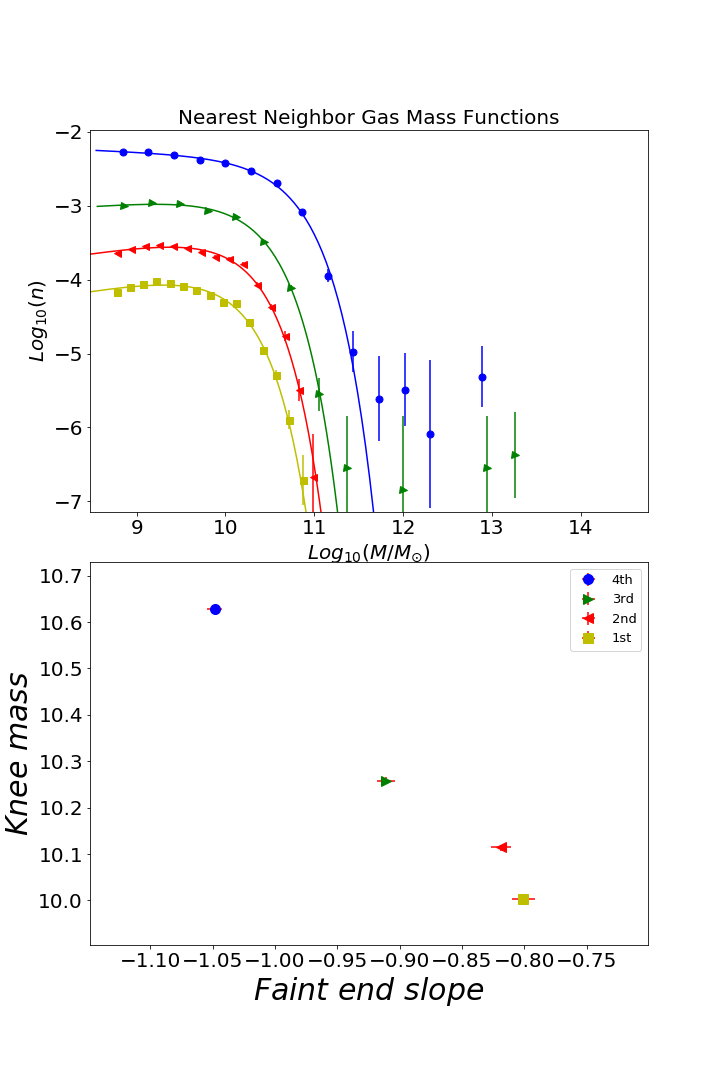
\includegraphics[width=\columnwidth]{./pics/quartilesGas.png}
    \caption{\textbf{Upper side}: Schechter fits of each gas mass
      function for each environmental quartile (tendence) using the 3rd nearest
      neighbor definition.\textbf{Down side}: Knee-mass $m_\ast$ and
      the faint end slope $\alpha$ values obtained from the Schechter
      fits for each curve shown above.} 
    \label{fig:quartilesGas}
\end{figure}

% Tweb gas
\begin{figure}
	% To include a figure from a file named example.*
	% Allowable file formats are eps or ps if compiling using latex
	% or pdf, png, jpg if compiling using pdflatex
	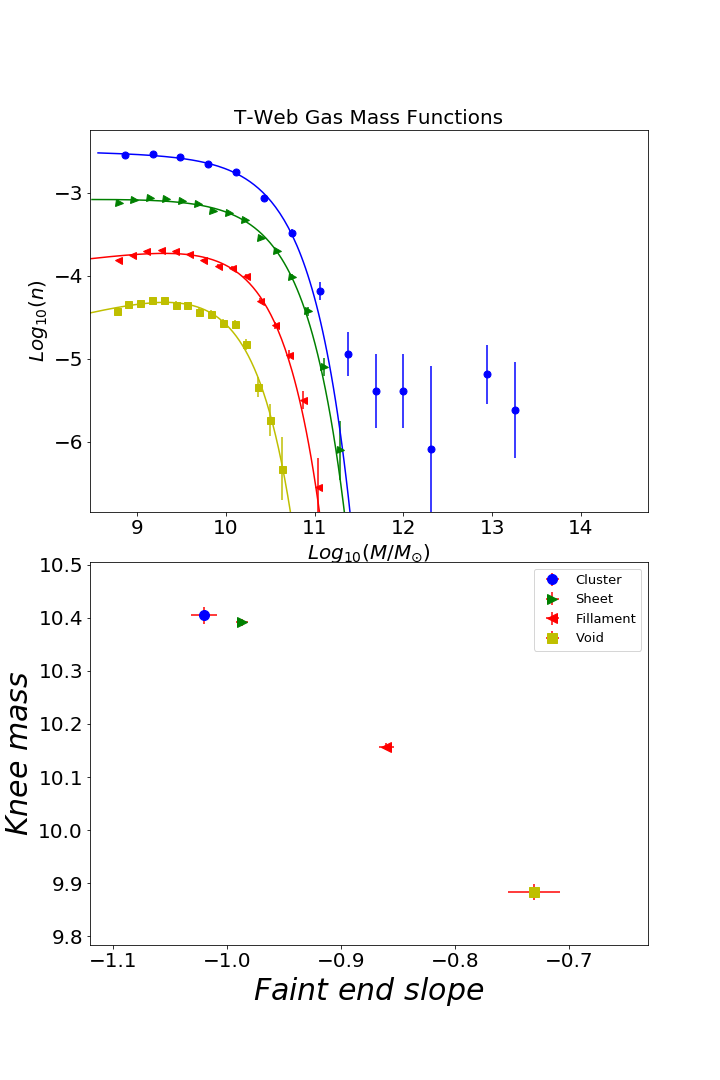
\includegraphics[width=\columnwidth]{./pics/T-Web_Gas.png}
    \caption{\textbf{Upper side}: Schechter fits of each gas mass
      function for each morphological environment characterized by the
      T-Web algorithm proposed by Forero et al.\textbf{Down side}:
      Knee-mass $m_\ast$ and the faint end slope $\alpha$ values
      obtained from the Schechter fits for each curve shown above.} 
    \label{fig:TwebGas}
\end{figure}

% Quartiles DM
\begin{figure}
	% To include a figure from a file named example.*
	% Allowable file formats are eps or ps if compiling using latex
	% or pdf, png, jpg if compiling using pdflatex
	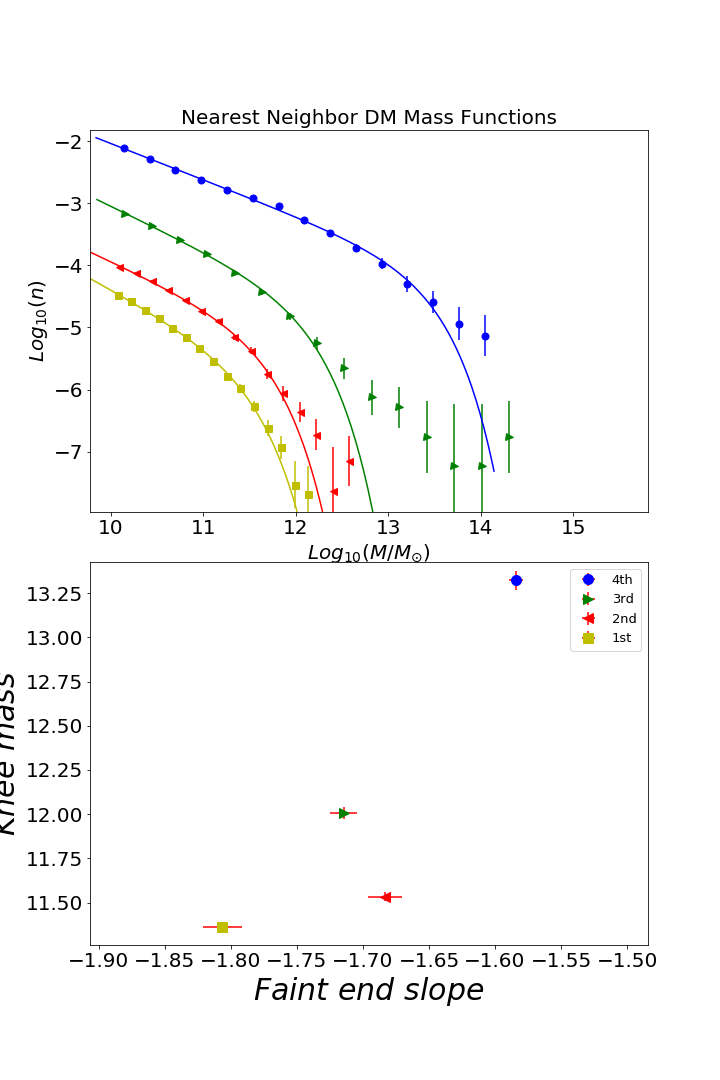
\includegraphics[width=\columnwidth]{./pics/quartilesDM.png}
    \caption{Similar to figure \ref{fig:quartilesGas} using DM.} 
    \label{fig:quartilesDM}
\end{figure}

% Tweb DM
\begin{figure}
	% To include a figure from a file named example.*
	% Allowable file formats are eps or ps if compiling using latex
	% or pdf, png, jpg if compiling using pdflatex
	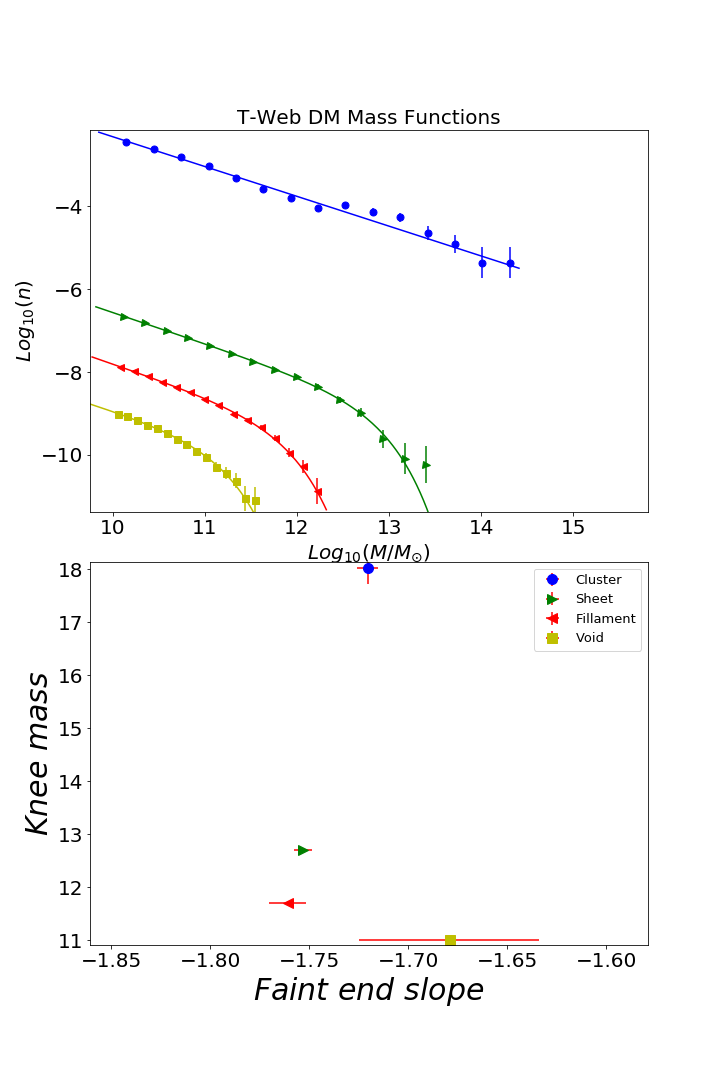
\includegraphics[width=\columnwidth]{./pics/T-Web_DM.png}
    \caption{Similar to figure \ref{fig:TwebGas} using DM.} 
    \label{fig:TwebDM}
\end{figure}

% Quartiles Stellar
\begin{figure}
	% To include a figure from a file named example.*
	% Allowable file formats are eps or ps if compiling using latex
	% or pdf, png, jpg if compiling using pdflatex
	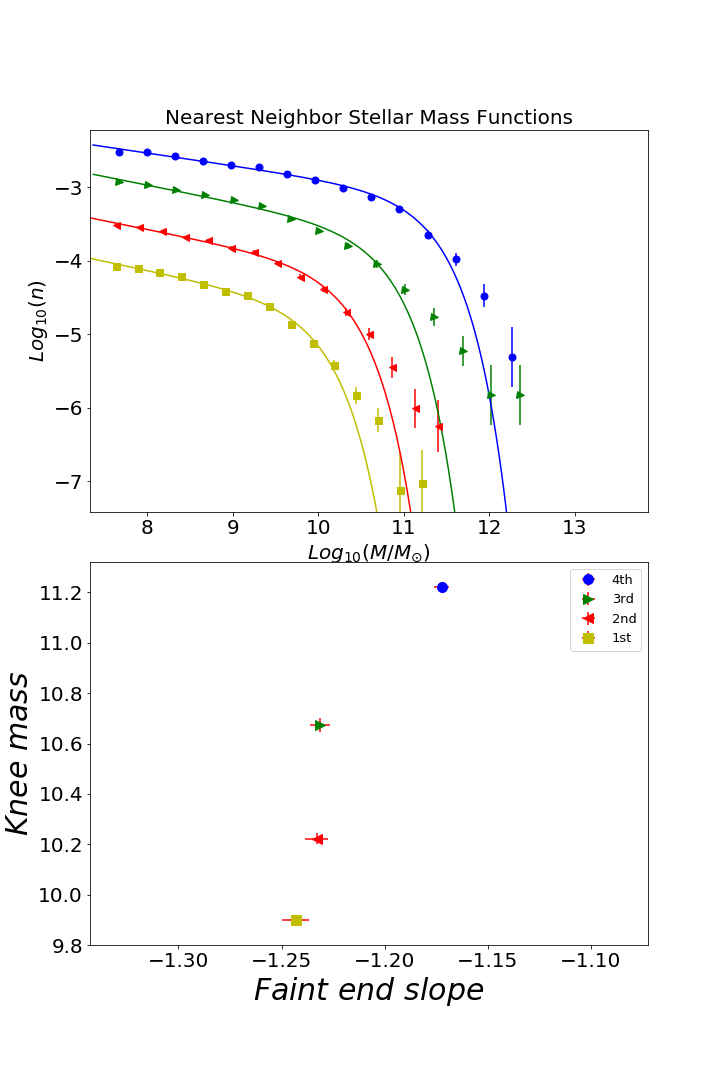
\includegraphics[width=\columnwidth]{./pics/quartilesSellar.png}
    \caption{Similar to figure \ref{fig:quartilesGas} using stellar mass} 
    \label{fig:quartilesStellar}
\end{figure}

% Tweb Stellar
\begin{figure}
	% To include a figure from a file named example.*
	% Allowable file formats are eps or ps if compiling using latex
	% or pdf, png, jpg if compiling using pdflatex
	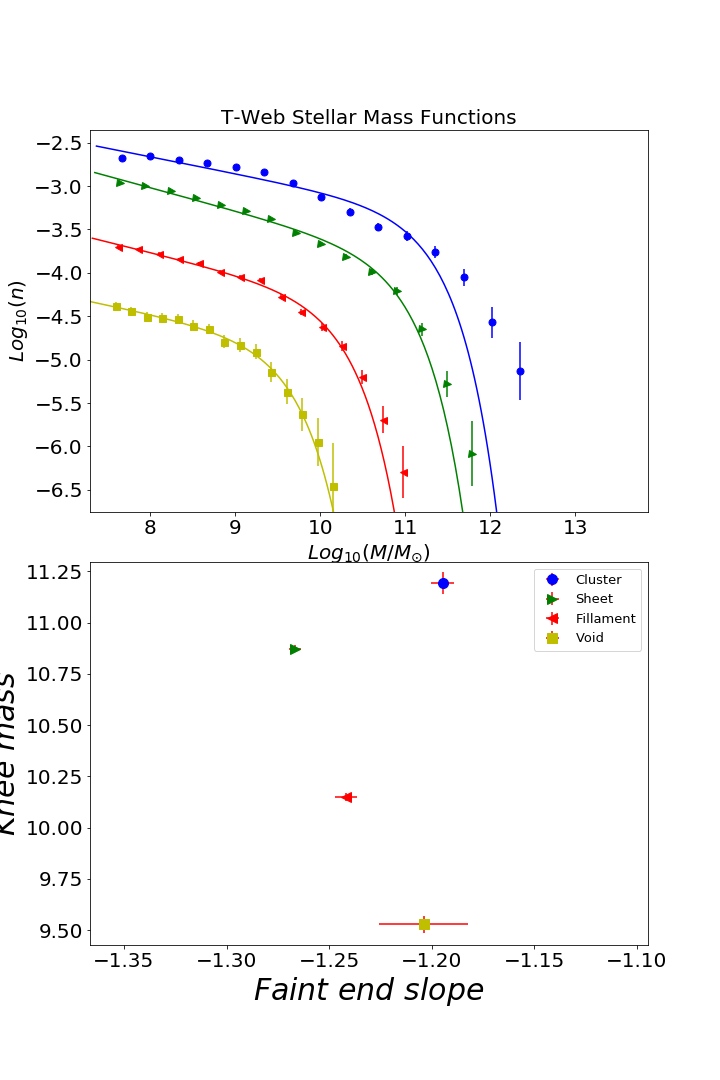
\includegraphics[width=\columnwidth]{./pics/T-Web_Stellar.png}
    \caption{Similar to figure \ref{fig:TwebGas} using stellar mass} 
    \label{fig:TwebStellar}
\end{figure}

% Quartiles BH
\begin{figure}
	% To include a figure from a file named example.*
	% Allowable file formats are eps or ps if compiling using latex
	% or pdf, png, jpg if compiling using pdflatex
	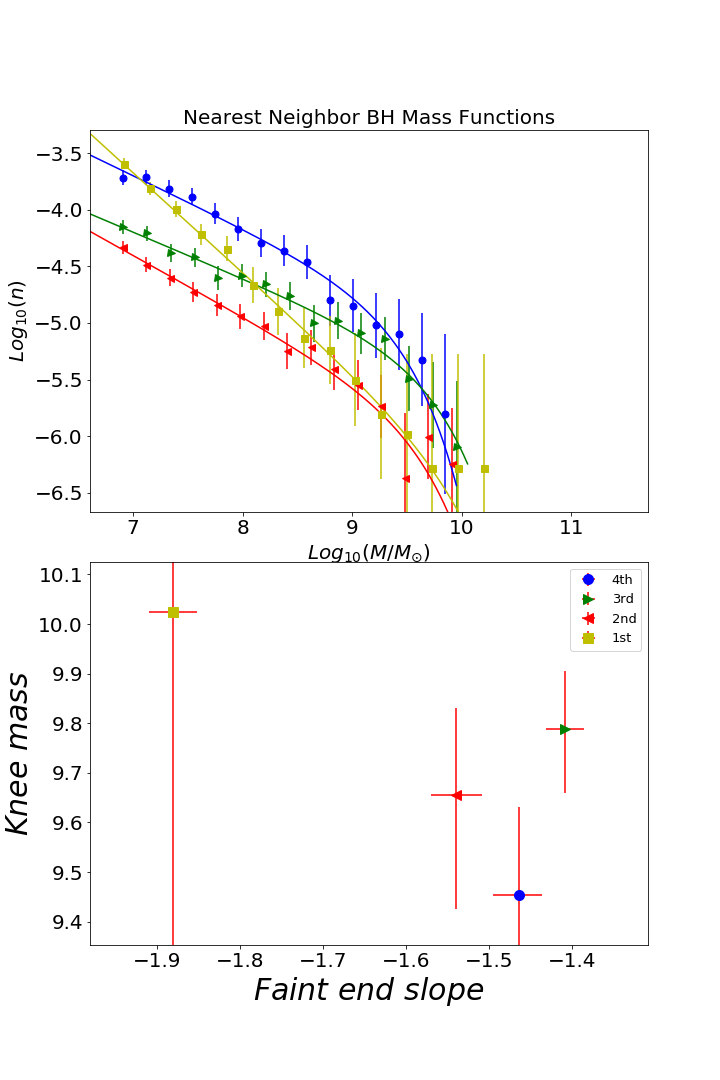
\includegraphics[width=\columnwidth]{./pics/quartilesBH.png}
    \caption{Similar to figure \ref{fig:quartilesGas} using BHs mass.} 
    \label{fig:quartilesBH}
\end{figure}

% Tweb BH
\begin{figure}
	% To include a figure from a file named example.*
	% Allowable file formats are eps or ps if compiling using latex
	% or pdf, png, jpg if compiling using pdflatex
	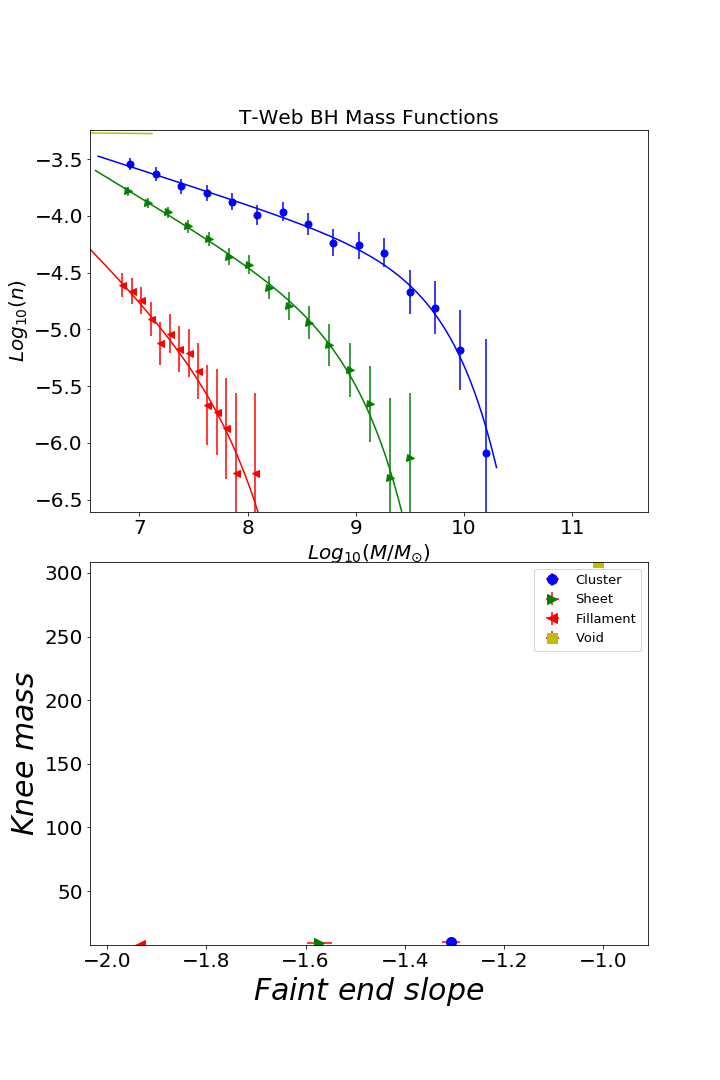
\includegraphics[width=\columnwidth]{./pics/T-Web_BH.png}
    \caption{Similar to figure \ref{fig:TwebGas} using BHs mass.} 
    \label{fig:TwebBH}
\end{figure}

% Example table
\begin{table}
	\centering
	\caption{This is an example table. Captions appear above each table.
	Remember to define the quantities, symbols and units used.}
	\label{tab:example_table}
	\begin{tabular}{lccr} % four columns, alignment for each
		\hline
		A & B & C & D\\
		\hline
		1 & 2 & 3 & 4\\
		2 & 4 & 6 & 8\\
		3 & 5 & 7 & 9\\
		\hline
	\end{tabular}
\end{table}


\section{Conclusions}

The last numbered section should briefly summarise what has been done, and describe
the final conclusions which the authors draw from their work.

\section*{Acknowledgements}

The Acknowledgements section is not numbered. Here you can thank helpful
colleagues, acknowledge funding agencies, telescopes and facilities used etc.
Try to keep it short.

%%%%%%%%%%%%%%%%%%%%%%%%%%%%%%%%%%%%%%%%%%%%%%%%%%

%%%%%%%%%%%%%%%%%%%% REFERENCES %%%%%%%%%%%%%%%%%%

\bibliographystyle{mnras}
\bibliography{references}


%%%%%%%%%%%%%%%%%%%%%%%%%%%%%%%%%%%%%%%%%%%%%%%%%%


%%%%%%%%%%%%%%%%% APPENDICES %%%%%%%%%%%%%%%%%%%%%

\appendix

\section{Some extra material}

If you want to present additional material which would interrupt the flow of the main paper,
it can be placed in an Appendix which appears after the list of references.

%%%%%%%%%%%%%%%%%%%%%%%%%%%%%%%%%%%%%%%%%%%%%%%%%%

\bsp	% typesetting comment
\label{lastpage}


\end{document}

% End of mnras_template.tex
